\documentclass[12pt]{article}
 \usepackage[margin=1in]{geometry} 
\usepackage{amsmath}
\usepackage[utf8]{inputenc}
%\usepackage[ utf8 ]{inputenc}
\usepackage[magyar]{babel}
\newcommand{\N}{\mathbb{N}}
\newcommand{\Z}{\mathbb{Z}}
\usepackage{t1enc}
\usepackage{listings}
\usepackage{placeins}
\usepackage{caption}
\usepackage{color}

\usepackage{graphicx}
\usepackage{placeins}
\usepackage{float}
\usepackage{subfigure}


\usepackage[utf8]{inputenc}
\usepackage[T1]{fontenc}
\title{Véletlen fizikai folyamatok, negyedik házi feladat}
\author{Horváth Bendegúz}




\begin{document}
\lstset{frame=tb,
  language=python,
  aboveskip=3mm,
  belowskip=3mm,
  showstringspaces=false,
  columns=flexible,
  basicstyle={\small\ttfamily},
  numbers=none,
  numberstyle=\tiny\color{gray},
  keywordstyle=\color{blue},
  commentstyle=\color{dkgreen},
  stringstyle=\color{mauve},
  breaklines=true,
  breakatwhitespace=true,
  tabsize=3
}

\maketitle
\section*{Szimuláció}
A program megírásához a $\texttt{Python}$ nyelvet használtam, a számításokat és a vizualizációt is ebben a környezetben hajtottam végre.

Előszőr importáltam a szükséges csomagokat, és a személyre szabott $\beta k a^2 $ adatomat.
\begin{lstlisting}
%pylab inline
i = 1
l = [0.14, 0.28, 0.56, 1.15] 
betaka2 = l[i]
\end{lstlisting}
Utána definiáltam egy redukált $\Delta E$, azért redukált, mert leosztottam $\beta k a^2$-tel. Az argumentumai $n$ és $n\pm 1$.
\begin{lstlisting}
def DeltaE(n, npm1):
    return 1/2*(npm1**2-n**2)
\end{lstlisting}
Ezután implementáltam a szimulációs lépést, ami egy egész számot vár bemenetként, a részecske helyzetét.
\begin{lstlisting}
def SimulationStep(n):
    r = random.random(1)
    direction = ((r-1/2)/abs(r-1/2))
    npm1 = int(n+direction)
    if DeltaE(n, npm1) < 0:
        n = npm1
    else:
        rand = random.random(1)
        if rand < exp(-betaka2*DeltaE(n, npm1)):
            n = npm1
        else:
            n = n
    return (n)
\end{lstlisting}
A szimuláció végrehajtása a \texttt{SimulationStep(n)} függvény folyamatos meghívásásával történik. Egy \texttt{steps} nevű tömbhöz minden egyes lépés után hozzácsatoltam a részecske helyzetét.
\begin{lstlisting}
temp = 0
steps = []
for i in range(1000000):
    n = temp
    steps.append(temp)
    temp = SimulationStep(n)
steps.append(temp)
print(temp)

Output: 3
\end{lstlisting}

A számításokat a beépített függvényekkel végeztem el, a részecske távolról indítva 0 körüli egyensúlyi helyzetbe megy át a relaxációs idő alatt. Én a rácspont 200. pontjából indítottam, és a relaxációs időt a 0 pont elérésének vettem. Így az átlagokat a relaxációs idő letelte után számoltam.
\begin{lstlisting}
for t in range(len(steps)):
    if steps[t] == 0:
        print(t)
        break
Output: 390
\end{lstlisting}
Egy összefoglaló táblázat a szimulációkról:

\begin{center}
\begin{tabular}{ |c|c|c|c|c|c|c|} 
 \hline
 $\beta k a^2$& lépések száma & $\langle x \rangle$ & $\langle x^2\rangle$& $\langle x^2\rangle - \langle x \rangle ^2$& relaxációs idő [lépés] & indulás helye [a] \\ \hline
 0.14 & 1000000 & 0.00850842&7.21865690 &7.21858450 &403&200\\ \hline
 0.28 & 1000000 & 0.00716580 & 3.59012874 &3.59007739 &392&200\\ \hline
 0.56 & 1000000&-0.01202176&1.78234280& 1.78219827&397&200\\ \hline
 1.15&1000000&0.00061125&0.86798166&0.86798129&405&200 \\
 \hline
\end{tabular}
\end{center}
A táblázatban lévő adatokból az látszik, hogy az átlag a $\beta ka^2$ növelésével egyre jobban közelít a 0-hoz, valamint a $\beta ka^2$ növelésével fordítottan arányos  a szórásnégyzet. A kísérleteket sokszor elvégezve ugyanezekkel a bemeneti paraméterekkel 5 tizedesjegyig ezeket az értékeket kaptam. A relaxációs idő és az indulás helyének adataiból is feltételezhetünk valami összefüggést a kettő között, és feltételezhetjük, hogy nem függ a hőmérséklettől. Ennek az összefüggésnek a vizsgálata érdekében csináltam még pár szimulációt.
\begin{center}
\begin{tabular}{ |c|c|} 
 \hline
indulás helye &relaxációs idő [lépés] \\ \hline
400&842\\ \hline
600& 1227\\ \hline
1000&2062\\ \hline
0& 0\\ \hline
-400&825\\ \hline
-600&1193\\ \hline
-1000& 1967\\ \hline

\end{tabular}
\end{center}

\begin{figure}[H]
\centering
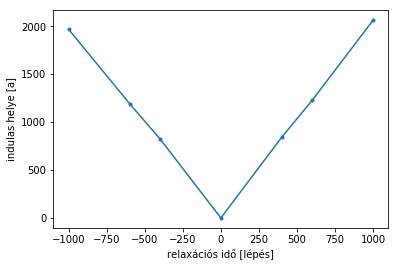
\includegraphics[width = 60mm]{relax}
\caption{A relaxációs idő az induláshelyének függvényében. Feltételezhtető egy $\tau = 2\cdot | x_0|$ összefüggés.}
\end{figure}
\begin{figure}[H]
\centering
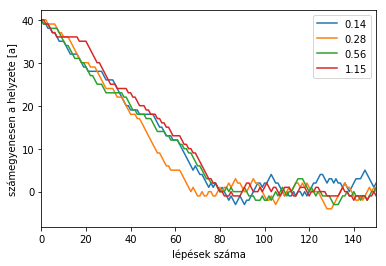
\includegraphics[width = 60mm, height = 35mm]{all.png}
\caption{Ábrázolva különböző $\beta ka^2$ értékek mellett a részecske helyzete a lépések számának függvényében.}
\end{figure}

A valószínűségi eloszlás függvényt közelíthetjük a relatívgyakoriságokkal. Egyensúlyi helyzetben vizsgáljuk meg, hogy mi lehet $P^{(e)}(n)$. A bemeneti paraméterek: lépésszám = 1000000, $\beta ka^2 = 0.56$.
\begin{center}
\begin{tabular}{ |c|c|}
\hline
 n&$P^{(e)}(n)$ \\ \hline
 -8& 0\\ \hline
-7&0\\ \hline
-6&$1.799\cdot 10^{-5}$ \\ \hline
-5&0.0002519 \\ \hline
-4&0.00355199\\ \hline
-3&0.02477197\\ \hline
-2& 0.098436 \\ \hline
-1&0.2256807\\ \hline
0& 0.29858670 \\ \hline
1& 0.22449777 \\ \hline
2&0.096939903 \\ \hline
3&0.0235609 \\ \hline
4& 0.00336399663\\ \hline
5&0.000306999\\ \hline
6&$3.09999\cdot 10^{-5}$\\ \hline
7&$9.999\cdot 10^{-7}$\\ \hline
8& 0\\ \hline

\end{tabular}
\end{center}
\newpage
 A relatív gyakoriságokat is egy függvénnyel számoltam:
 \begin{lstlisting}
 def relative_frequency(lst, element):
    return lst.count(element) / float(len(lst))
 \end{lstlisting}
Ábrázolva a az értékeket:

\begin{figure}[H]
\centering
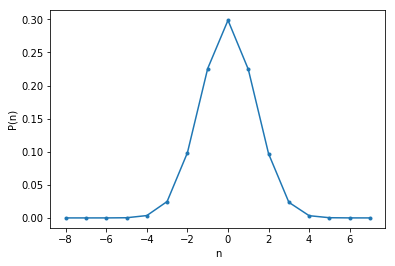
\includegraphics[width = 80 mm]{pn}
\caption{A $P^{(e)}(n)$ értékek, összekötve egyenes szakaszokkal.}
\end{figure}

Az ábrán látható pontok összekötve egy Gauss-görbe szerű függvényt adnak. Próbálkoztam valahogyan kombinálva a paramétereket egy olyan függvényt készíteni, ami a legjobban illik a pontjainkra.
Az illesztett függvény meglepően jól fedi a pontjainkat.
\begin{figure}[H]
\centering
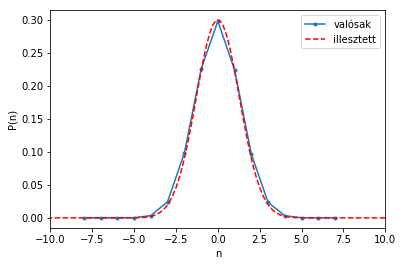
\includegraphics[width = 80 mm]{pnill}
\caption{A $P^{(e)}(n)$ értékek, és a ráillesztett függvény .}
\end{figure}


Az legjobban illeszkedő függvény a következő alakú volt:
$$P^{(e)}(n) = \frac{1}{\pi\sqrt{2\cdot \beta k a^2}}e^{-\frac{n^2}{\pi\sqrt{2\cdot \beta k a^2}}}$$
\end{document}